\documentclass[10pt,a4paper]{article}
\usepackage[margin=2.0cm]{geometry}
\usepackage[T1]{fontenc}
\usepackage{lmodern}
\usepackage{amsmath,amssymb}
\usepackage{booktabs}
\usepackage{graphicx}
\usepackage{caption}
\usepackage{tikz}
\usetikzlibrary{positioning,arrows.meta,fit}
\usepackage[hidelinks]{hyperref}
\captionsetup{font=small,labelfont=bf}
\setlength{\parskip}{3pt}

\title{Dual-scale neural-operator correction of station winds in Northern Norway:\\
input groups, a dual-scale GNO decoder, and a gridded check against MET Nordic}
\author{Windcast project, track A}
\date{November 2026}

\begin{document}
\maketitle

\begin{abstract}
We correct 10\,m wind forecasts at 99 stations in Northern Norway (leads 0--66\,h) by learning the
residual between the observation and the mean of several forecast models, with networks that see
forecast fields, terrain and time but no observations and no station coordinates. Combining global
(IFS, AIFS) and regional (MEPS, AROME-Arctic) models is the decisive choice: their uncorrected mean is
7.0\,\% better than the IFS+AIFS mean, and a point-wise MLP on top reaches $-10.2$\,\%. The proposed
dual-scale design (a global and a regional neural-operator encoder, each read at the target point by
its own graph neural operator, fused by one linear projection) overfits as specified and is worse
than the uncorrected mean ($-5.8$\,\%). Smaller encoders, a zero-initialised output and an MLP head
recover most of the gap ($-9.6$\,\%); adding potential-temperature and mountain-wind features gives
$-10.0\pm0.0$\,\%, level with but not better than the MLP, and the GNO readout performs like a
bilinear one. Shrinking the encoders further (width 8, $4\times8$ modes) changes nothing. Doubling the
training period (1236 instead of 592 runs, tested April--November 2026) improves every model by about
2 points without changing the ranking: point-wise MLP $-12.9$\,\%, best dual-scale model $-12.0$\,\%,
and with more data the physical features no longer help. Adding 79 Swedish and Finnish stations to
training improves the Norwegian test stations by only 0.1--0.4 points. Applied on the 1\,km MET Nordic grid, all corrections move slightly away from the
analysis (+0.6 to +7.4\,\%); but at the stations the analysis is itself beaten by the corrected
forecasts, so MET Nordic wind, which follows MEPS, is not a suitable reference for station-trained
corrections.
\end{abstract}

%=====================================================================
\section{Introduction}
Global models (IFS, AIFS; 0.25$^\circ$) resolve neither fjords nor ridges, and regional models
(MEPS, AROME-Arctic; 2.5\,km) retain systematic near-surface errors, so 10\,m wind forecasts in
Northern Norway carry location- and flow-dependent biases. Track~A of the windcast project learns a
correction at the stations that transfers to unseen locations: the networks see neither observations
nor station coordinates, so the same weights apply wherever forecasts and terrain are available. We
ask (i) which combination of forecast models the correction should start from, and (ii) whether a
dual-scale neural-operator architecture, keeping regional fields at 2.5\,km and aggregating each scale
around the target point with a graph neural operator, adds skill over point-wise models.

%=====================================================================
\section{Data and evaluation}\label{sec:data}
\paragraph{Forecasts.} IFS and AIFS (ECMWF open data, 0.25$^\circ$), GFS (0.25$^\circ$, used only in
the earlier four-model group), MEPS and AROME-Arctic (MET Norway, 2.5\,km), initialised at 00
and 12\,UTC from 1~March 2024 to 12~September 2025 (1019 runs), leads 0--66\,h every 6\,h
($L=12$). At a station, global models are interpolated bilinearly; regional models take the
nearest native 2.5\,km cell. On grids, global models are on a common 0.25$^\circ$ grid
(49$\times$121 points, 62--74$^\circ$N, 6--36$^\circ$E); regional models are on a common 2.5\,km
grid of the project's Lambert azimuthal plane (299$\times$345 cells) or, for the mixed group,
averaged onto the 0.25$^\circ$ grid. Runs in which any model of a group is missing are dropped.

\paragraph{Observations and terrain.} Hourly 10\,m wind at 99 MET Norway (Frost) stations in
Nordland, Troms and Finnmark. Each station is described by 28 descriptors computed on a 1\,km
terrain grid (elevation, slope, aspect, topographic position, sub-grid roughness, sector
shelter $S_x$ at 1 and 10\,km, distance to the coast, land fraction, \ldots).

\paragraph{Splits.} Training on runs initialised 1~March--31~December 2024, validation
January--March 2025, test 1~April--12~September 2025. In addition the stations are split into
five spatial groups by $k$-means on their coordinates (28, 17, 14, 20 and 20 stations). Each of
five folds trains on four groups and keeps the epoch with the lowest validation loss on the
held-out group; its test predictions for the held-out group are stitched into one test set in
which every station is predicted by a model that never saw it.

\paragraph{Extended period.} Section~\ref{sec:longer} repeats the main models on a longer sample
period, 1~March 2024 to 14~November 2026 (1875 runs; with the Norway-wide Frost download for 2026):
training 1~March 2024--31~December 2025 (1236 runs), validation January--March 2026 (180), test
1~April--14~November 2026 (452). Stations, spatial groups and all settings are unchanged. All other
sections use the original period.

\paragraph{Metric.} Vector RMSE, $\sqrt{\overline{|\hat{\mathbf u}-\mathbf u_{\rm obs}|^2}}$, over
station, run and lead. All numbers are computed on the same 367\,427 test samples (all input
groups available, observation present) and reported as the relative change with respect to the
IFS+AIFS mean (3.489\,m\,s$^{-1}$). Results are the mean over three seeds unless stated; $\pm$ is
the standard deviation across seeds.

%=====================================================================
\section{Methods}\label{sec:methods}
\subsection{Residual formulation}
For an input group of $M$ models with station forecasts $\mathbf f_m(x,t)$ the baseline is
the mean $\bar{\mathbf f}(x,t)=\frac1M\sum_m \mathbf f_m(x,t)$, and the networks predict
\begin{equation}
\Delta\hat{\mathbf u}(x,t) \approx \mathbf u_{\rm obs}(x,t)-\bar{\mathbf f}(x,t),\qquad
\hat{\mathbf u}=\bar{\mathbf f}+\Delta\hat{\mathbf u},
\end{equation}
trained with the mean squared error of the vector residual divided by its training standard
deviation, at the training stations only. This is equivalent to predicting the wind with a fixed
skip connection to the model mean.

\subsection{Reference models}
\textbf{Point-wise MLP.} A network (two hidden layers of 128, GELU; 22.5\,k parameters)
on the 28 terrain descriptors (z-scored over the stations), the $2M$ forecast wind components,
the mean wind speed, the upwind shelter at 1 and 10\,km for the mean wind direction, and five
time features (lead, hour and day of year as sine/cosine). \textbf{SFNO/FNO + MLP.} The same
head, additionally fed with 32 latent channels of a neural operator (spherical or planar Fourier
neural operator, width 64, $16\times32$ modes, 4 layers) run on the group grid (10\,m wind,
2\,m temperature and MSLP of each model, plus the time channels) and read bilinearly at the
station.

\subsection{Dual-scale GNO}
Following the design document, the global and regional forecasts are encoded separately and
fused only at the target point (Fig.~\ref{fig:arch}):
\begin{align}
Z_g &= E_g(X_g,\tau), & Z_r &= E_r(X_r,\tau),\\
h_g(x) &= \mathrm{GNO}_g(Z_g,x;r_g), & h_r(x) &= \mathrm{GNO}_r(Z_r,x;r_r),\\
\Delta\hat{\mathbf u}(x,t) &= W\,[\,h_g,\ h_r,\ T(x),\ \mathbf f(x,t),\ \tau(t)\,] + b, &&
\end{align}
where $E_g$ is an SFNO on the IFS+AIFS 0.25$^\circ$ grid and $E_r$ an FNO on the MEPS+AROME-Arctic
2.5\,km grid (each width 64, $16\times32$ modes, 4 layers, 32 output channels);
$T(x)$ are the 28 terrain descriptors, $\mathbf f(x,t)$ the eight forecast wind components and
$\tau(t)$ the time features. The GNO is a kernel integral over the grid points $y$ within radius
$r$ of $x$,
\begin{equation}
\mathrm{GNO}(Z,x;r)=\frac{1}{|N_r(x)|}\sum_{y\in N_r(x)} k\!\left(\tfrac{y-x}{r},\ \tfrac{|y-x|}{r},\ Z(y)\right)\odot Z(y),
\end{equation}
where the kernel $k$ is an MLP ($35\rightarrow64\rightarrow64\rightarrow32$) that sees only the
relative displacement and the source features, never absolute coordinates; each scale is
normalised over its own neighbours. With $r_g=60$\,km and $r_r=10$\,km a station has 34--47
global and 47--52 regional neighbours. A control replaces
both GNOs by bilinear sampling of $Z_g$ and $Z_r$ at $x$. The design deliberately has no fusion
MLP or attention: one linear map produces the residual.

\begin{figure}[t]
\centering
\begin{tikzpicture}[font=\footnotesize, node distance=4mm and 6mm,
  box/.style={draw, rounded corners=2pt, align=center, minimum height=8mm, inner sep=3pt},
  in/.style={box, fill=gray!10}, enc/.style={box, fill=blue!8}, gno/.style={box, fill=orange!12},
  out/.style={box, fill=green!10}, arr/.style={-{Latex[length=2mm]}}]
\node[in] (xg) {Global forecasts $X_g$\\IFS + AIFS, 0.25$^\circ$\\$u_{10},v_{10},T_2,p_{\rm msl}$};
\node[in, below=6mm of xg] (xr) {Regional forecasts $X_r$\\MEPS + AROME, 2.5\,km\\$u_{10},v_{10},T_2,p_{\rm msl}$};
\node[enc, right=of xg] (eg) {Global encoder $E_g$\\SFNO $\rightarrow$ 32 ch};
\node[enc, right=of xr] (er) {Regional encoder $E_r$\\FNO $\rightarrow$ 32 ch};
\node[gno, right=of eg] (gg) {GNO$_g$\\$r_g=60$ km};
\node[gno, right=of er] (gr) {GNO$_r$\\$r_r=10$ km};
\node[in, below=6mm of gr] (pt) {Point features at $x$: terrain (28),\\forecast winds (8), time (5)\\{[}+ $\theta$ (7), mountain wind (15){]}};
\node[out, right=8mm of gg, yshift=-7mm] (fu) {Concatenate\\+ linear projection\\{[}control: MLP head{]}};
\node[out, right=of fu] (o) {$\Delta\hat{\mathbf u}(x,t)$\\+ four-model mean};
\draw[arr] (xg) -- (eg); \draw[arr] (xr) -- (er);
\draw[arr] (eg) -- (gg); \draw[arr] (er) -- (gr);
\draw[arr] (gg) -- (fu); \draw[arr] (gr) -- (fu); \draw[arr] (pt.east) -| (fu.south);
\draw[arr] (fu) -- (o);
\end{tikzpicture}
\caption{Dual-scale GNO. Each encoder also receives the five time channels. The GNOs aggregate
each latent field around the target point $x$ using relative displacements only, so the model can
be evaluated at any point. Brackets mark the additions tested in Section~\ref{sec:results}.}
\label{fig:arch}
\end{figure}

\subsection{Potential-temperature and mountain-wind features}
Stability and terrain-forced flow are not visible in the 10\,m fields alone, so 22 optional point
features are derived from the forecasts and the 1\,km terrain (Table~\ref{tab:phys}). Like the
terrain descriptors they exist at any 1\,km cell. Upper-air variables come from IFS and AIFS
(bilinear), boundary-layer height, cloud cover and 2\,m temperature from MEPS and AROME-Arctic
(nearest cell).

\begin{table}[t]
\centering\small
\caption{Potential-temperature ($\theta$) and mountain-wind features. $\theta=T(1000/p)^{0.2857}$;
$N$ is the bulk Brunt--V\"ais\"al\"a frequency of the surface--850\,hPa layer; $H$ is the relief
within 10\,km.}\label{tab:phys}
\begin{tabular}{@{}lp{0.78\linewidth}@{}}
\toprule
$\theta$ group (7) & $\theta_{2\rm m}$ of the global models; $\theta_{850}-\theta_{2\rm m}$; $\theta_{700}-\theta_{850}$; $N$;
$\theta_{2\rm m}$ at the station height (regional $T_{2\rm m}$, pressure reduced from MSLP); $\theta_{850}-\theta_{2\rm m,st}$ (valley cold pools); $\log_{10}$ boundary-layer height\\
Mountain group (15) & $u_{850}, v_{850}$; $\log_{10}$ Froude number $U_{850}/(NH)$; 10\,m speed; upwind shelter (1, 10\,km);
upslope wind $\mathbf U_{10}\cdot\nabla z$ (1\,km) and $\mathbf U_{850}\cdot\nabla z$ (ridge scale, $\sigma=5$\,km); sine of solar elevation;
clear-sky fraction; slope insolation; anabatic vector (insolation$\times\nabla z$); katabatic vector (clear sky$\times$night$\times(-\nabla z)$)\\
\bottomrule
\end{tabular}
\end{table}

\subsection{Training}
All models: AdamW (weight decay $10^{-4}$), one-cycle learning rate with maximum $10^{-5}$, batch
16 runs (all stations and one lead per sample), 40 epochs, best validation epoch kept.

%=====================================================================
\section{Results}\label{sec:results}
\subsection{Input groups}
Table~\ref{tab:groups} compares the input groups. Mixing global and regional models is by far the
largest effect: the uncorrected four-model mean improves on either pair alone (IFS+AIFS 0\,\%,
MEPS+AROME $-2.3$\,\%, mixed $-7.0$\,\%), and every correction model inherits this advantage.
Replacing GFS by AIFS in the four-model group improves all three networks by 0.5--0.7 points for
every seed, consistent with a model-subset analysis in which GFS added nothing once IFS was present.
Neural operators help only when the input is global alone (SFNO $-4.4$\,\% vs MLP $-3.3$\,\%); with
regional models in the input the point-wise MLP is best, and on the native 2.5\,km grid the operator
gain is within 0.3 points (using nine rather than four regional fields made no consistent
difference). The bar for the dual-scale model is therefore the mixed-group MLP at $-10.2$\,\%.

\begin{table}[t]
\centering\small
\caption{Test RMSE change (\%) relative to the IFS+AIFS mean, by input group (3 seeds, 5 spatial
folds). ``Uncorrected'' is the plain mean of the group's models.}\label{tab:groups}
\begin{tabular}{@{}lcccc@{}}
\toprule
Input group & Uncorrected & MLP & SFNO + MLP & FNO + MLP\\
\midrule
IFS + AIFS (0.25$^\circ$) & +0.0 & -3.3 $\pm$ 0.3 & -4.4 $\pm$ 0.8 & -3.0 $\pm$ 0.4 \\
MEPS + AROME-Arctic (2.5 km) & -2.3 & -5.5 $\pm$ 0.1 & -5.8 $\pm$ 0.1 & -4.6 $\pm$ 0.1 \\
IFS + AIFS + MEPS + AROME-Arctic & -7.0 & \textbf{-10.2 $\pm$ 0.2} & -9.4 $\pm$ 0.1 & -9.2 $\pm$ 0.4 \\
IFS + GFS + MEPS + AROME-Arctic (old) & -6.3 & -9.5 $\pm$ 0.2 & -8.9 $\pm$ 0.2 & -8.7 $\pm$ 0.4 \\
\bottomrule
\end{tabular}
\end{table}

\subsection{The dual-scale GNO as specified overfits}
The design as specified (5.1\,M parameters, linear output) is worse than doing nothing: $-5.8$\,\%
with the GNO readout and $-6.1$\,\% with bilinear readout, against $-7.0$\,\% for the uncorrected
four-model mean (Table~\ref{tab:dual}). Figure~\ref{fig:curves} shows why. The training loss keeps
falling, but the validation loss on the held-out stations reaches its minimum after 5--10 epochs and
then rises, whereas the 22\,k-parameter MLP improves until the end. With about 600 training runs the
two encoders can memorise run-specific field patterns. A second, smaller defect is the random
initialisation of the output projection, which starts the model above the zero-correction loss.

\begin{figure}[t]
\centering
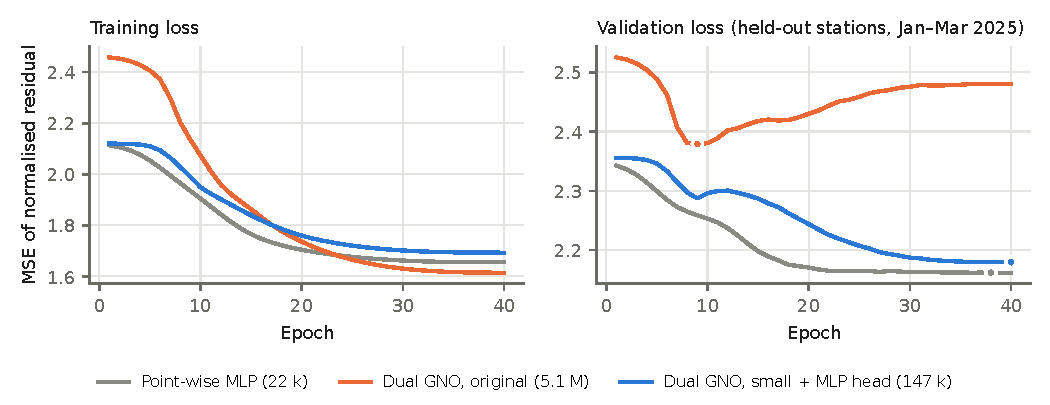
\includegraphics[width=\linewidth]{figs/fig_curves.pdf}
\caption{Training and validation loss for fold 0, seed 0. Dots mark the epoch that is kept.}
\label{fig:curves}
\end{figure}

\subsection{Capacity, regularisation and the output head}
Three changes were tested on seed 0 and the best carried to three seeds (Table~\ref{tab:dual},
Fig.~\ref{fig:bars}). (i) \emph{Smaller encoders} (width 16, $8\times16$ modes; 117\,k parameters)
with a zero-initialised output reach $-8.2$\,\%, now better than the uncorrected mean. Dropout on the
latent features and stronger weight decay change nothing. (ii) \emph{An MLP head} in place of the
linear projection, i.e.\ the same head as the reference MLP, adds another 1.0--1.3 points (seed 0): $-9.6\pm0.2$\,\%
with the GNO. With the original encoder size the MLP head gives only $-8.6$\,\%, so both changes are
needed. (iii) \emph{The GNO and bilinear readouts are equivalent} in every pairing (differences
$\le0.2$ points), so the neighbourhood aggregation does not yet contribute beyond reading the latent
field at the point. (iv) \emph{Even smaller encoders} (width 8 and/or $4\times8$ modes, 61--89\,k
parameters, best configuration with $\theta$ + mountain features, seed 0) give $-9.8$ to $-10.0$\,\%,
the same as width 16 with $8\times16$ modes: encoder size is no longer the bottleneck.

\begin{table}[t]
\centering\small
\caption{Dual-scale models, test RMSE change (\%) relative to the IFS+AIFS mean. Best epoch: mean over
folds and seeds of the epoch kept (of 40). Small encoders: width 16, $8\times16$ Fourier modes.}
\label{tab:dual}
\footnotesize
\begin{tabular}{@{}lrrcr@{}}
\toprule
Model & Parameters & Best epoch & Seeds & $\Delta$RMSE (\%)\\
\midrule
\multicolumn{5}{l}{\emph{References (mix input group)}} \\
\quad Uncorrected four-model mean & -- & -- & -- & -7.0 \\
\quad Point-wise MLP (mix) & 23 k & 27 & 3 & -10.2 $\pm$ 0.2 \\
\quad SFNO + MLP (mix, 0.25$^\circ$) & 607 k & 20 & 3 & -9.4 $\pm$ 0.1 \\
\midrule
\multicolumn{5}{l}{\emph{Original size (PDF design, linear head)}} \\
\quad Dual NO + bilinear readout & 5.09 M & 9 & 3 & -6.1 $\pm$ 1.0 \\
\quad Dual NO + GNO & 5.11 M & 9 & 3 & -5.8 $\pm$ 0.7 \\
\quad Dual NO + GNO + $\theta$ + mountain & 5.11 M & 12 & 3 & -4.6 $\pm$ 0.3 \\
\midrule
\multicolumn{5}{l}{\emph{Small encoders, zero-initialised output}} \\
\quad Dual NO + bilinear readout & 100 k & 13 & 1 & -8.4 \\
\quad Dual NO + GNO & 117 k & 12 & 1 & -8.2 \\
\quad \quad + dropout 0.3, weight decay $10^{-2}$ (bilinear) & 100 k & 13 & 1 & -8.4 \\
\quad \quad + dropout 0.3, weight decay $10^{-2}$ (GNO) & 117 k & 17 & 1 & -8.2 \\
\midrule
\multicolumn{5}{l}{\emph{MLP head instead of the linear projection: original size}} \\
\quad Dual NO + bilinear readout & 5.12 M & 11 & 1 & -8.8 \\
\quad Dual NO + GNO & 5.14 M & 13 & 1 & -8.6 \\
\midrule
\multicolumn{5}{l}{\emph{MLP head: small encoders}} \\
\quad Dual NO + bilinear readout & 130 k & 27 & 1 & -9.4 \\
\quad Dual NO + GNO & 147 k & 25 & 3 & -9.6 $\pm$ 0.2 \\
\quad Dual NO + GNO + $\theta$ & 148 k & 26 & 3 & -9.4 $\pm$ 0.1 \\
\quad Dual NO + GNO + mountain & 149 k & 24 & 3 & -9.5 $\pm$ 0.2 \\
\quad Dual NO + GNO + $\theta$ + mountain & 150 k & 24 & 3 & -10.0 $\pm$ 0.0 \\
\quad \quad width 16, $4\times8$ modes & 89 k & 32 & 1 & -9.8 \\
\quad \quad width 8, $8\times16$ modes & 76 k & 29 & 1 & -10.0 \\
\quad \quad width 8, $4\times8$ modes & 61 k & 28 & 1 & -10.0 \\
\bottomrule
\end{tabular}
\end{table}

\begin{figure}[t]
\centering
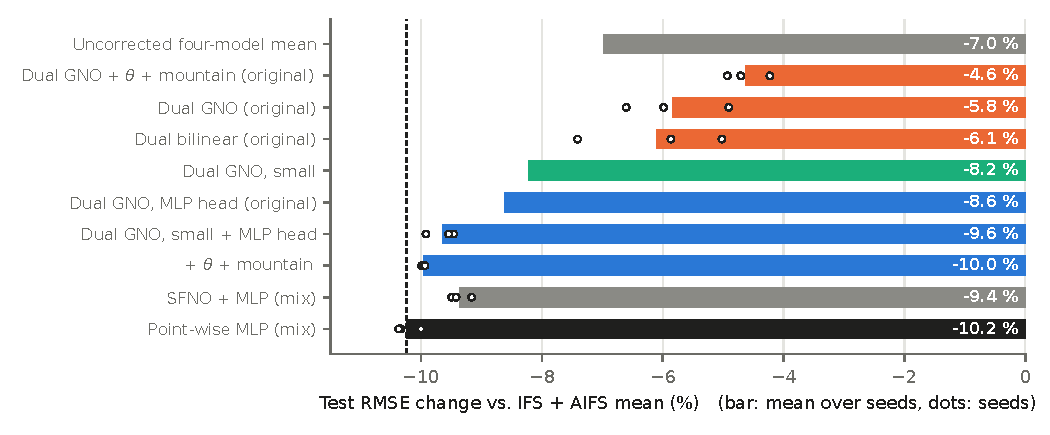
\includegraphics[width=\linewidth]{figs/fig_bars.pdf}
\caption{Summary of the dual-scale experiments against the references. The dashed line marks the
point-wise MLP. Orange: design as specified; green: small encoders; blue: MLP head.}
\label{fig:bars}
\end{figure}

\subsection{Potential-temperature and mountain-wind features}
On the overfitting original model the 22 physical features made matters worse ($-4.6$\,\%). On the
small model with MLP head, each group alone is neutral (\,$\theta$: $-9.4\pm0.1$\,\%, mountain:
$-9.5\pm0.2$\,\%, none: $-9.6\pm0.2$\,\%), while both together give $-10.0\pm0.0$\,\%, the best and most
stable dual-scale result. The combination matters physically: the Froude number, anabatic and
katabatic terms are products of stability and terrain-relative flow, and the network uses them
jointly. The best dual-scale model is level with the point-wise MLP ($-10.2\pm0.2$\,\%) within the seed
spread, but not better.

\subsection{Lead time and station groups}
The ranking is the same at all leads (Fig.~\ref{fig:leadgroup}, left): the corrections remove
0.09--0.14\,m\,s$^{-1}$ from the four-model mean at every lead, and the best dual-scale model tracks
the point-wise MLP within 0.02\,m\,s$^{-1}$. Across held-out station groups (right) the gains relative to the
four-model mean range from $-1.4$ to $-5.4$\,\%, depending on group and model. Group~0 (28 stations) is where the
operator-based models are weakest: the SFNO model is slightly worse than the uncorrected mean there,
and the dual-scale model recovers only part of the MLP's gain, which suggests that the latent fields
carry information that does not transfer to that part of the domain.

\begin{figure}[t]
\centering
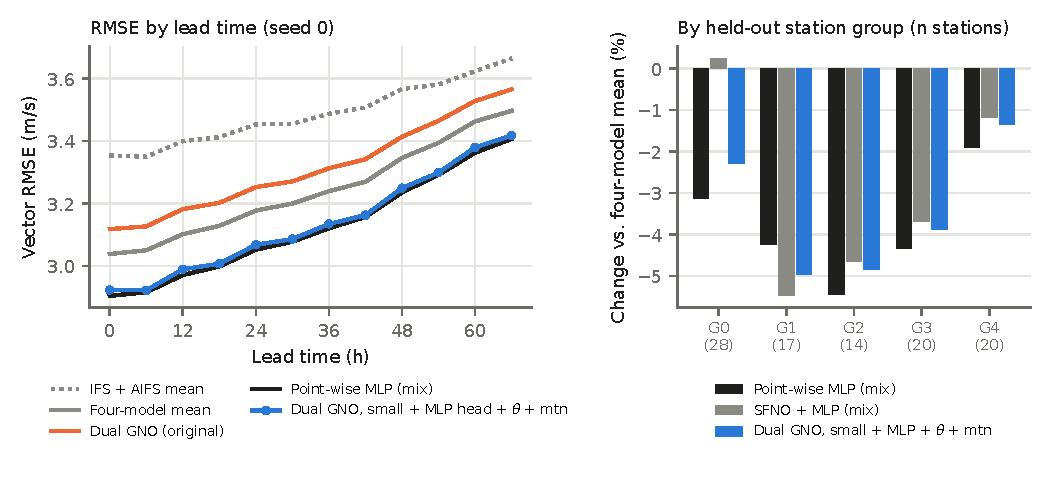
\includegraphics[width=\linewidth]{figs/fig_lead_group.pdf}
\caption{Left: vector RMSE by lead time (seed 0). Right: RMSE change relative to the four-model mean
for each held-out station group (seed 0; number of stations in brackets).}
\label{fig:leadgroup}
\end{figure}

\subsection{Doubling the training period}\label{sec:longer}
With about 600 training runs every larger model overfitted, so the main models were retrained on the
extended period (Section~\ref{sec:data}; 1236 training runs, test April--November 2026, 509\,729 test
samples, IFS+AIFS mean 3.701\,m\,s$^{-1}$). Table~\ref{tab:longer} lists the results next to the
original period; the two test periods differ, so only changes in ranking and differences between
models can be compared across the columns.
\begin{itemize}\itemsep1pt
\item \emph{Every correction gains about 2 points}, while the uncorrected four-model mean gains 0.75.
The point-wise MLP goes from $-10.2$ to $-12.9$\,\%, the best dual-scale model from $-10.0$ to
$-12.0$\,\%. The ranking does not change: the MLP stays best, now by 0.8 points.
\item \emph{The physical features no longer help}: with and without $\theta$ + mountain features the
small dual-scale model reaches $-12.0$\,\%. On the shorter period they mattered only in combination,
which suggests that they mainly compensated for the lack of data.
\item \emph{GNO and bilinear readouts remain equivalent} ($-12.0$ vs $-11.9$\,\%, seed 0).
\item \emph{The original-size models still lose}, though by less: the design as specified reaches
$-6.7$\,\% and its MLP-head variant $-10.4$\,\%, both still below the small encoders.
\end{itemize}

\begin{table}[t]
\centering\small
\caption{Original and extended period, test RMSE change (\%) relative to the IFS+AIFS mean of each test
set. Seeds refer to the extended period; the original-period values are from Table~\ref{tab:dual}.
Small dual-scale models: width 16, $8\times16$ modes, zero-initialised MLP head.}\label{tab:longer}
\begin{tabular}{@{}lccc@{}}
\toprule
Model & Seeds & Original period & Extended period\\
\midrule
Uncorrected four-model mean & -- & -7.0 & -7.8 \\
Point-wise MLP & 3 & -10.2 $\pm$ 0.2 & \textbf{-12.9 $\pm$ 0.1} \\
SFNO + MLP (0.25$^\circ$) & 3 & -9.4 $\pm$ 0.1 & -11.3 $\pm$ 0.3 \\
Dual NO + GNO, as specified & 1 & -5.8 $\pm$ 0.7 & -6.7 \\
Dual NO + GNO, original size, MLP head & 1 & -8.6 & -10.4 \\
Dual NO + GNO, small & 3 & -9.6 $\pm$ 0.2 & -12.0 $\pm$ 0.2 \\
Dual NO + GNO, small, $\theta$ + mountain & 3 & -10.0 $\pm$ 0.0 & -12.0 $\pm$ 0.2 \\
Dual NO + bilinear, small, $\theta$ + mountain & 1 & -- & -11.9 \\
\bottomrule
\end{tabular}
\end{table}

\paragraph{Additional Swedish and Finnish training stations.} To test whether more stations help in
the same way as more runs, 79 SMHI and FMI stations (41 Swedish, 38 Finnish, $>$50\,\% hourly
coverage) were added to the training set of the five Norwegian folds; evaluation stays on the same 99
Norwegian stations, each again predicted by a model that never saw it. The gain is small: point-wise MLP
$-12.9\to-13.0$\,\% (3 seeds), dual-scale with $\theta$ + mountain $-12.0\to-12.4$\,\% (3 seeds),
dual-scale without them $-11.8\to-12.1$\,\% (seed 0) and SFNO + MLP $-11.3\to-12.2$\,\% (seed 0
against the three-seed mean). The operator
models benefit more than the MLP, but only the dual-scale gain exceeds the seed spread, and barely.
Inland Swedish and Finnish stations have weaker winds and smaller residuals (IFS+AIFS RMSE
2.7\,m\,s$^{-1}$ vs 3.7 in Norway) and do not cover the coastal and mountain terrain where the Norwegian
errors arise. They are therefore not used further.

%=====================================================================
\subsection{Gridded evaluation against MET Nordic}\label{sec:metnordic}
Because no model sees station coordinates or observations, the trained networks can be applied at
any point. We applied them on the Troms{\o}--Senja part of the MET Nordic v4 analysis grid
(1\,km): 14\,180 land cells, every second cell in both directions, over the 328 test runs
(April--September 2025, all 12 leads). Every input is built at the cell exactly as at a station:
the forecast winds of the four models, the 28 terrain descriptors of the cell (z-scored with the
station statistics of training), and the potential-temperature and mountain-wind features with the
cell elevation in place of the station height. Each configuration is the mean of its 15 trained
models (5 folds $\times$ 3 seeds); the $\pm$ values use the per-seed means of the five fold models.
The reference is the MET Nordic analysis 10\,m wind at the valid time.

\begin{table}[t]
\centering\small
\caption{Left: vector RMSE against the MET Nordic analysis on the 1\,km grid (14\,180 land cells,
328 test runs, all leads) and its change relative to the four-model mean, for all cells and for
cells more than 10\,km from any station (88\,\% of the cells). Right: the same models, and the
MET Nordic analysis itself, against the observations at the 40 stations inside the grid
(153\,997 samples; three-seed mean).}\label{tab:metnordic}
\begin{tabular}{@{}lccc|c@{}}
\toprule
& \multicolumn{3}{c|}{vs.\ MET Nordic, grid} & vs.\ observations\\
Model & RMSE (m\,s$^{-1}$) & $\Delta$ all (\%) & $\Delta$ $>$10\,km (\%) & RMSE (m\,s$^{-1}$)\\
\midrule
IFS + AIFS mean & 2.933 & +41.9 & +41.9 & 3.897 \\
MEPS + AROME-Arctic mean & 1.983 & -4.0 & -3.9 & 3.695 \\
Four-model mean & 2.067 & +0.0 & +0.0 & 3.563 \\
\midrule
Point-wise MLP & 2.134 & +3.3 $\pm$ 1.1 & +3.0 & 3.457 \\
SFNO + MLP & 2.119 & +2.5 $\pm$ 1.5 & +2.4 & 3.463 \\
Dual GNO, as specified & 2.220 & +7.4 $\pm$ 2.1 & +7.4 & 3.638 \\
Dual GNO, small + MLP head & 2.080 & +0.6 $\pm$ 1.3 & +0.5 & 3.479 \\
\quad + $\theta$ + mountain & 2.127 & +2.9 $\pm$ 0.1 & +2.9 & 3.458 \\
\midrule
MET Nordic analysis & -- & -- & -- & 3.495 \\
\bottomrule
\end{tabular}
\end{table}

Table~\ref{tab:metnordic} and Fig.~\ref{fig:metnordic} show a result that is the opposite of the
station evaluation: against MET Nordic, every correction \emph{increases} the error relative to the
four-model mean (from $+0.6$\,\% for the small dual-scale model to $+7.4$\,\% for the design as
specified), and the plain MEPS + AROME-Arctic mean is closest to the analysis ($-4.0$\,\%). The
disagreement is largest close to the stations, where the corrections are largest, and decreases
with distance (Fig.~\ref{fig:metnordic}, right). The station check explains why this is not
evidence against the corrections. At the 40 stations inside the grid, the MET Nordic analysis
itself differs from the observed wind by 3.49\,m\,s$^{-1}$, only 1.9\,\% less than the
four-model mean \emph{forecast} (3.56\,m\,s$^{-1}$), and the station-corrected forecasts at leads
of 0--66\,h (MLP 3.46, dual-scale with $\theta$ + mountain 3.46\,m\,s$^{-1}$) are closer to the
observations than the analysis is. The MET Nordic wind field is close to MEPS (the regional
pair is 1.98\,m\,s$^{-1}$ from it, the observations 3.49\,m\,s$^{-1}$), so it does not contain
the station-scale signal that the corrections learn, and moving towards the observations moves
away from the analysis.

Two conclusions follow. First, MET Nordic is not a suitable reference for verifying 10\,m wind
corrections trained on station observations; it measures consistency with a MEPS-like field, not
accuracy. Second, within that limitation the gridded check is still informative about behaviour
away from the stations: the corrections do not blow up anywhere in the domain, the
design-as-specified model departs most from the analysis everywhere (consistent with its
overfitting), and the small dual-scale model is the most conservative off-station
($-0.2$ to $+0.2$\,\% beyond 10\,km). Verification away from the stations will need independent
observations, for example the withheld Swedish and Finnish stations or a cross-check against
Netatmo-type networks.

\begin{figure}[t]
\centering
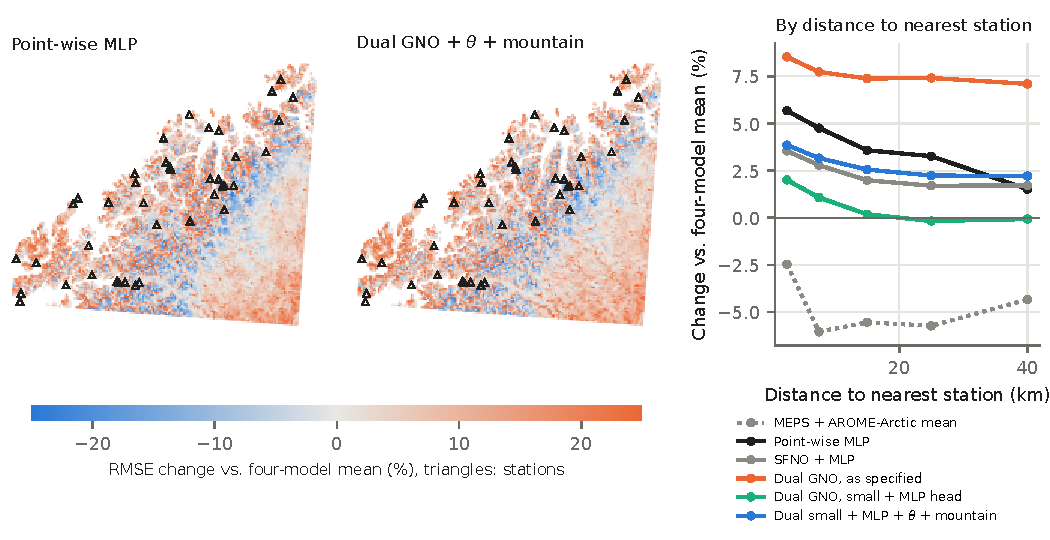
\includegraphics[width=\linewidth]{figs/fig_metnordic.pdf}
\caption{Gridded evaluation against MET Nordic. Left and centre: change in RMSE relative to the
four-model mean at each 2\,km land cell for the point-wise MLP and the best dual-scale model
(blue: closer to MET Nordic; orange: further). Triangles are stations. Right: the change as a
function of distance to the nearest station.}
\label{fig:metnordic}
\end{figure}

%=====================================================================
\section{Discussion}\label{sec:discussion}
\paragraph{What carries the skill.} The largest gain is the choice of forecast models in the
baseline; the networks add a further 3 points on top of the four-model mean, and among them the
point-wise MLP on local forecast winds, terrain and time is as good as any operator. The dual-scale
model only reached this level with the same non-linear head, and its GNO readout was not
distinguishable from a bilinear one. A single linear projection cannot form the terrain--flow
interactions (e.g.\ shelter times wind direction) that dominate the residual; in the specified model
they can only arise inside encoders that do not see terrain, learned from about 600 training runs
with 5\,M parameters, which leads to overfitting rather than a lack of capacity. The extended period
confirms that data, not architecture, limits the skill: twice as many training runs add about 2 points
to every model, more than any architectural change, whereas 79 extra stations in a different climate
add at most 0.4.

\paragraph{Limitations.} The test periods cover April--September 2025 and April--November 2026, so
winter stability regimes (where $\theta$ features should matter most) are seen only in validation. The ablations on seed 0
alone have a seed spread of up to 1--2 points for the large models. The global encoder sees four
fields per model; upper-air fields enter only through the point features.

\paragraph{Next steps.} (1) Give the GNO kernel terrain information at the query and source points,
so that the neighbourhood aggregation can become terrain-aware. (2) Sweep $r_g$ and $r_r$ (the design
document's sweep) now that the model no longer overfits, together with the wind-aligned GNO frame.
(3) Test over a full annual cycle, including winter, and add training stations with Norwegian-like
terrain (Tr{\o}ndelag, the west coast) rather than inland Swedish and Finnish ones. (4) Ensemble the point-wise MLP and the dual-scale
model, whose errors are partly independent across station groups.

%=====================================================================
\section{Conclusions}
\begin{itemize}\itemsep1pt
\item The input group IFS + AIFS + MEPS + AROME-Arctic gives the best baseline ($-7.0$\,\%) and the
best corrected forecast ($-10.2$\,\% with a point-wise MLP); GFS can be dropped.
\item The dual-scale GNO as specified (two NO encoders, dual-radius GNO, linear fusion) overfits and
is worse than the uncorrected mean ($-5.8$\,\%).
\item Small encoders, a zero-initialised output and an MLP head make it competitive ($-9.6$\,\%);
with potential-temperature and mountain-wind features it reaches $-10.0\pm0.0$\,\%, level with but
not better than the point-wise MLP.
\item Doubling the training period improves every model by about 2 points (point-wise MLP
$-12.9$\,\%, best dual-scale model $-12.0$\,\%) without changing the ranking; the physical features
then no longer help, and further shrinking the encoders changes nothing.
\item Adding 79 Swedish and Finnish training stations improves the Norwegian stations by only
0.1--0.4 points; they are not used.
\item GNO and bilinear readouts are equivalent so far; terrain-aware kernels and a radius sweep are
the natural next experiments.
\item On the 1\,km MET Nordic grid the corrections stay bounded everywhere but move away from the
analysis, which tracks MEPS and is no closer to the station observations than the corrected
forecasts. Off-station verification needs independent observations.
\end{itemize}

\end{document}
